\documentclass[english, 11 pt, class=article, crop=false]{standalone}
\usepackage[T1]{fontenc}
%\renewcommand*\familydefault{\sfdefault} % For dyslexia-friendly text
\usepackage{lmodern} % load a font with all the characters
\usepackage{geometry}
\geometry{verbose,paperwidth=16.1 cm, paperheight=24 cm, inner=2.3cm, outer=1.8 cm, bmargin=2cm, tmargin=1.8cm}
\setlength{\parindent}{0bp}
\usepackage{import}
\usepackage[subpreambles=false]{standalone}
\usepackage{amsmath}
\usepackage{amssymb}
\usepackage{esint}
\usepackage{babel}
\usepackage{tabu}
\makeatother
\makeatletter

\usepackage{titlesec}
\usepackage{ragged2e}
\RaggedRight
\raggedbottom
\frenchspacing

% Norwegian names of figures, chapters, parts and content
\addto\captionsenglish{\renewcommand{\figurename}{Figur}}
\makeatletter
\addto\captionsenglish{\renewcommand{\chaptername}{Kapittel}}
\addto\captionsenglish{\renewcommand{\partname}{Del}}


\usepackage{graphicx}
\usepackage{float}
\usepackage{subfig}
\usepackage{placeins}
\usepackage{cancel}
\usepackage{framed}
\usepackage{wrapfig}
\usepackage[subfigure]{tocloft}
\usepackage[font=footnotesize,labelfont=sl]{caption} % Figure caption
\usepackage{bm}
\usepackage[dvipsnames, table]{xcolor}
\definecolor{shadecolor}{rgb}{0.105469, 0.613281, 1}
\colorlet{shadecolor}{Emerald!15} 
\usepackage{icomma}
\makeatother
\usepackage[many]{tcolorbox}
\usepackage{multicol}
\usepackage{stackengine}

\usepackage{esvect} %For vectors with capital letters

% For tabular
\usepackage{array}
\usepackage{multirow}
\usepackage{longtable} %breakable table

% Ligningsreferanser
\usepackage{mathtools}
\mathtoolsset{showonlyrefs}

% index
\usepackage{imakeidx}
\makeindex[title=Indeks]

%Footnote:
\usepackage[bottom, hang, flushmargin]{footmisc}
\usepackage{perpage} 
\MakePerPage{footnote}
\addtolength{\footnotesep}{2mm}
\renewcommand{\thefootnote}{\arabic{footnote}}
\renewcommand\footnoterule{\rule{\linewidth}{0.4pt}}
\renewcommand{\thempfootnote}{\arabic{mpfootnote}}

%colors
\definecolor{c1}{cmyk}{0,0.5,1,0}
\definecolor{c2}{cmyk}{1,0.25,1,0}
\definecolor{n3}{cmyk}{1,0.,1,0}
\definecolor{neg}{cmyk}{1,0.,0.,0}

% Lister med bokstavar
\usepackage[inline]{enumitem}

\newcounter{rg}
\numberwithin{rg}{chapter}
\newcommand{\reg}[2][]{\begin{tcolorbox}[boxrule=0.3 mm,arc=0mm,colback=blue!3] {\refstepcounter{rg}\phantomsection \large \textbf{\therg \;#1} \vspace{5 pt}}\newline #2  \end{tcolorbox}\vspace{-5pt}}

\newcommand\alg[1]{\begin{align} #1 \end{align}}

\newcommand\eks[2][]{\begin{tcolorbox}[boxrule=0.3 mm,arc=0mm,enhanced jigsaw,breakable,colback=green!3] {\large \textbf{Eksempel #1} \vspace{5 pt}\\} #2 \end{tcolorbox}\vspace{-5pt} }

\newcommand{\st}[1]{\begin{tcolorbox}[boxrule=0.0 mm,arc=0mm,enhanced jigsaw,breakable,colback=yellow!12]{ #1} \end{tcolorbox}}

\newcommand{\spr}[1]{\begin{tcolorbox}[boxrule=0.3 mm,arc=0mm,enhanced jigsaw,breakable,colback=yellow!7] {\large \textbf{Språkboksen} \vspace{5 pt}\\} #1 \end{tcolorbox}\vspace{-5pt} }

\newcommand{\sym}[1]{\colorbox{blue!15}{#1}}

\newcommand{\info}[2]{\begin{tcolorbox}[boxrule=0.3 mm,arc=0mm,enhanced jigsaw,breakable,colback=cyan!6] {\large \textbf{#1} \vspace{5 pt}\\} #2 \end{tcolorbox}\vspace{-5pt} }

\newcommand\algv[1]{\vspace{-11 pt}\begin{align*} #1 \end{align*}}

\newcommand{\regv}{\vspace{5pt}}
\newcommand{\mer}{\textsl{Merk}: }
\newcommand{\mers}[1]{{\footnotesize \mer #1}}
\newcommand\vsk{\vspace{11pt}}
\newcommand\vs{\vspace{-11pt}}
\newcommand\vsb{\vspace{-16pt}}
\newcommand\sv{\vsk \textbf{Svar} \vspace{4 pt}\\}
\newcommand\br{\\[5 pt]}
\newcommand{\figp}[1]{../fig/#1}
\newcommand\algvv[1]{\vs\vs\begin{align*} #1 \end{align*}}
\newcommand{\y}[1]{$ {#1} $}
\newcommand{\os}{\\[5 pt]}
\newcommand{\prbxl}[2]{
\parbox[l][][l]{#1\linewidth}{#2
	}}
\newcommand{\prbxr}[2]{\parbox[r][][l]{#1\linewidth}{
		\setlength{\abovedisplayskip}{5pt}
		\setlength{\belowdisplayskip}{5pt}	
		\setlength{\abovedisplayshortskip}{0pt}
		\setlength{\belowdisplayshortskip}{0pt} 
		\begin{shaded}
			\footnotesize	#2 \end{shaded}}}

\renewcommand{\cfttoctitlefont}{\Large\bfseries}
\setlength{\cftaftertoctitleskip}{0 pt}
\setlength{\cftbeforetoctitleskip}{0 pt}

\newcommand{\bs}{\\[3pt]}
\newcommand{\vn}{\\[6pt]}
\newcommand{\fig}[1]{\begin{figure}
		\centering
		\includegraphics[]{\figp{#1}}
\end{figure}}

\newcommand{\figc}[2]{\begin{figure}
		\centering
		\includegraphics[]{\figp{#1}}
		\caption{#2}
\end{figure}}

\newcommand{\sectionbreak}{\clearpage} % New page on each section

\newcommand{\nn}[1]{
\begin{equation}
	#1
\end{equation}
}

% Equation comments
\newcommand{\cm}[1]{\llap{\color{blue} #1}}

\newcommand\fork[2]{\begin{tcolorbox}[boxrule=0.3 mm,arc=0mm,enhanced jigsaw,breakable,colback=yellow!7] {\large \textbf{#1 (forklaring)} \vspace{5 pt}\\} #2 \end{tcolorbox}\vspace{-5pt} }
 
%colors
\newcommand{\colr}[1]{{\color{red} #1}}
\newcommand{\colb}[1]{{\color{blue} #1}}
\newcommand{\colo}[1]{{\color{orange} #1}}
\newcommand{\colc}[1]{{\color{cyan} #1}}
\definecolor{projectgreen}{cmyk}{100,0,100,0}
\newcommand{\colg}[1]{{\color{projectgreen} #1}}

% Methods
\newcommand{\metode}[2]{
	\textsl{#1} \\[-8pt]
	\rule{#2}{0.75pt}
}

%Opg
\newcommand{\abc}[1]{
	\begin{enumerate}[label=\alph*),leftmargin=18pt]
		#1
	\end{enumerate}
}
\newcommand{\abcs}[2]{
	\begin{enumerate}[label=\alph*),start=#1,leftmargin=18pt]
		#2
	\end{enumerate}
}
\newcommand{\abcn}[1]{
	\begin{enumerate}[label=\arabic*),leftmargin=18pt]
		#1
	\end{enumerate}
}
\newcommand{\abch}[1]{
	\hspace{-2pt}	\begin{enumerate*}[label=\alph*), itemjoin=\hspace{1cm}]
		#1
	\end{enumerate*}
}
\newcommand{\abchs}[2]{
	\hspace{-2pt}	\begin{enumerate*}[label=\alph*), itemjoin=\hspace{1cm}, start=#1]
		#2
	\end{enumerate*}
}

% Oppgaver
\newcommand{\opgt}{\phantomsection \addcontentsline{toc}{section}{Oppgaver} \section*{Oppgaver for kapittel \thechapter}\vs \setcounter{section}{1}}
\newcounter{opg}
\numberwithin{opg}{section}
\newcommand{\op}[1]{\vspace{15pt} \refstepcounter{opg}\large \textbf{\color{blue}\theopg} \vspace{2 pt} \label{#1} \\}
\newcommand{\ekspop}[1]{\vsk\textbf{Gruble \thechapter.#1}\vspace{2 pt} \\}
\newcommand{\nes}{\stepcounter{section}
	\setcounter{opg}{0}}
\newcommand{\opr}[1]{\vspace{3pt}\textbf{\ref{#1}}}
\newcommand{\oeks}[1]{\begin{tcolorbox}[boxrule=0.3 mm,arc=0mm,colback=white]
		\textit{Eksempel: } #1	  
\end{tcolorbox}}
\newcommand\opgeks[2][]{\begin{tcolorbox}[boxrule=0.1 mm,arc=0mm,enhanced jigsaw,breakable,colback=white] {\footnotesize \textbf{Eksempel #1} \\} \footnotesize #2 \end{tcolorbox}\vspace{-5pt} }
\newcommand{\rknut}{
Rekn ut.
}

%License
\newcommand{\lic}{\textit{Matematikken sine byggesteinar by Sindre Sogge Heggen is licensed under CC BY-NC-SA 4.0. To view a copy of this license, visit\\ 
		\net{http://creativecommons.org/licenses/by-nc-sa/4.0/}{http://creativecommons.org/licenses/by-nc-sa/4.0/}}}

%referances
\newcommand{\net}[2]{{\color{blue}\href{#1}{#2}}}
\newcommand{\hrs}[2]{\hyperref[#1]{\color{blue}\textsl{#2 \ref*{#1}}}}
\newcommand{\rref}[1]{\hrs{#1}{regel}}
\newcommand{\refkap}[1]{\hrs{#1}{kapittel}}
\newcommand{\refsec}[1]{\hrs{#1}{seksjon}}

\newcommand{\mb}{\net{https://sindrsh.github.io/FirstPrinciplesOfMath/}{MB}}


%line to seperate examples
\newcommand{\linje}{\rule{\linewidth}{1pt} }

\usepackage{datetime2}
%%\usepackage{sansmathfonts} for dyslexia-friendly math
\usepackage[]{hyperref}


\newcommand{\note}{Merk}
\newcommand{\notesm}[1]{{\footnotesize \textsl{\note:} #1}}
\newcommand{\ekstitle}{Eksempel }
\newcommand{\sprtitle}{Språkboksen}
\newcommand{\expl}{forklaring}

\newcommand{\vedlegg}[1]{\refstepcounter{vedl}\section*{Vedlegg \thevedl: #1}  \setcounter{vedleq}{0}}

\newcommand\sv{\vsk \textbf{Svar} \vspace{4 pt}\\}

%references
\newcommand{\reftab}[1]{\hrs{#1}{tabell}}
\newcommand{\rref}[1]{\hrs{#1}{regel}}
\newcommand{\dref}[1]{\hrs{#1}{definisjon}}
\newcommand{\refkap}[1]{\hrs{#1}{kapittel}}
\newcommand{\refsec}[1]{\hrs{#1}{seksjon}}
\newcommand{\refdsec}[1]{\hrs{#1}{delseksjon}}
\newcommand{\refved}[1]{\hrs{#1}{vedlegg}}
\newcommand{\eksref}[1]{\textsl{#1}}
\newcommand\fref[2][]{\hyperref[#2]{\textsl{figur \ref*{#2}#1}}}
\newcommand{\refop}[1]{{\color{blue}Oppgave \ref{#1}}}
\newcommand{\refops}[1]{{\color{blue}oppgave \ref{#1}}}
\newcommand{\refgrubs}[1]{{\color{blue}gruble \ref{#1}}}

\newcommand{\openmathser}{\openmath\,-\,serien}

% Exercises
\newcommand{\opgt}{\newpage \phantomsection \addcontentsline{toc}{section}{Oppgaver} \section*{Oppgaver for kapittel \thechapter}\vs \setcounter{section}{1}}


% Sequences and series
\newcommand{\sumarrek}{Summen av en aritmetisk rekke}
\newcommand{\sumgerek}{Summen av en geometrisk rekke}
\newcommand{\regnregsum}{Regneregler for summetegnet}

% Trigonometry
\newcommand{\sincoskomb}{Sinus og cosinus kombinert}
\newcommand{\cosfunk}{Cosinusfunksjonen}
\newcommand{\trid}{Trigonometriske identiteter}
\newcommand{\deravtri}{Den deriverte av de trigonometriske funksjonene}
% Solutions manual
\newcommand{\selos}{Se løsningsforslag.}
\newcommand{\se}[1]{Se eksempel på side \pageref{#1}}

%Vectors
\newcommand{\parvek}{Parallelle vektorer}
\newcommand{\vekpro}{Vektorproduktet}
\newcommand{\vekproarvol}{Vektorproduktet som areal og volum}


% 3D geometries
\newcommand{\linrom}{Linje i rommet}
\newcommand{\avstplnpkt}{Avstand mellom punkt og plan}


% Integral
\newcommand{\bestminten}{Bestemt integral I}
\newcommand{\anfundteo}{Analysens fundamentalteorem}
\newcommand{\intuf}{Integralet av utvalge funksjoner}
\newcommand{\bytvar}{Bytte av variabel}
\newcommand{\intvol}{Integral som volum}
\newcommand{\andordlindif}{Andre ordens lineære differensialligninger}



\begin{document}
	
	
\opgt

\op{antiderint}
\textbf{a)} Deriver funksjonen $ f(x)=4x^5 $.\os

\textbf{b)} Finn det bestemte integralet $ \int\limits_0^2 20 x^4 \, dx $.

\op{Fogf}
Relasjonen mellom en funksjon $ F(x) $ og $f(x) $ er at $ F'(x)=f(x) $. Videre er $ F(1)=1 $ og $ F(4)=9 $.\os

Finn det bestemte integralet \y{\int\limits_1^4 f(x) \, dx}.

\op{ecos2x}
\textbf{a)} Deriver funksjonen $ f(x)=e^{\cos^2 x} $.\os

\textbf{b)} Finn det ubestemte integralet \[ \int -\sin (2x)\, e^{\cos^2 x}\,dx \]\vs\vs

\op{visantider}
Vis at\os
\textbf{a)} $\displaystyle \int x(x+2)e^x \,dx = x^2 e^x + C $ \os

\textbf{b)} $\displaystyle \int -e^{x^2+\cos x} (-2 x+\sin x)\,dx= e^{\cos x+x^2}+C  $

\nes

\op{intsopg}
Finn integalene:\os
\begin{tabular}{@{}l l l l}	
\textbf{a)} $ \displaystyle \int \frac{3}{4 x} \,dx$ &\quad \textbf{b)} $ \displaystyle \int-\frac{7}{\cos^2 t}\,dt $ &\quad \textbf{c)} $ -4x^5 $ \\[20 pt]
\textbf{d)}\ $\displaystyle \int \cos(\pi x) \,dx$ & \quad
\textbf{e)} $\displaystyle \int 4e^{-4t} \,dt$ &\quad\textbf{f)} $ \displaystyle \int \left(2x^4\,dx - \frac{3}{x^{\frac{3}{2}}}\right) \,dx$ \\[20pt]
\textbf{g)} $\displaystyle \int \sqrt{x^5}\,dx $
\end{tabular} 
\newpage
\op{opgintbestmt}
Regn ut de bestemte integralene.\os
\abch{
\item $\displaystyle \int_{-1}^{1} \left(4x^3-x\right)\,dx $
\item  $\displaystyle \int_{0}^{\ln 2} e^{2x}\,dx $
}

\op{avcos}
Gjennomsnittet av en funksjon $ f(x) $ over et intervall $ [a, b] $ kan vi skrive som
\[ \frac{1}{b-a}\int\limits_a^b f(x)\,dx \]
Gitt et vilkårlig tall $ c $, vis at gjennomsnittet av $f(x)=\cos x+d  $ over intervallet $ [c, c+2\pi] $ er lik $ d $. 

\op{bytvaropg}
Finn integralene:\os

\begin{tabular}{@{}l l l}	
\textbf{a)} $\displaystyle \int xe^{x^2} \, dx  $ &\;\textbf{b)} $\displaystyle \int\limits_1^2 8xe^{2x^2-3}\,dx $ &\;\textbf{c)} $\displaystyle \int \tan x \, dx $ \\ \vspace{3pt} 
\textbf{d)} $ \displaystyle \int\limits_0^\frac{\pi}{3}\frac{\sin x}{\cos^3 x} \, dx $ &\;\textbf{e)} $ \displaystyle \int \frac{4x+5}{2x^2 + 5x}\,dx $
&\;\textbf{f)} $ \displaystyle \int \frac{3x+2}{3x^2 + 4x+3}\,dx $
\end{tabular} 

\op{trigint}
Anvend to av de trigonometriske identitetene og bytte av variabel to ganger for å finne integralet
\[ \int \sin (2x) e^{1-\cos^2 x}\,dx \]\vs


\op{delvisintopg}
Finn det bestemte/ubestemte integralet:\os
\begin{tabular}{@{}l l l}	
	\textbf{a)} $\displaystyle \int (x-1)\cos x \, dx$&\quad	\textbf{b)} $\displaystyle \int \sqrt{x}\ln x\,dx $ &\quad\textbf{c)} $\displaystyle \int\limits_1^e  \frac{\ln x}{x^2} $ 
\end{tabular}

\op{delvisintopg2}
Vis at
\[ \int \sin^2 x\,dx=\frac{1}{2}(x-\sin x \cos x)+C \]\vs

\newpage
\op{delbropsopg}
Finn det bestemte/ubestemte integralet:\os

\begin{tabular}{@{}l l l}	
	\textbf{a)} $ \displaystyle \int\limits_4^5 \frac{13-4x}{x^2-5x+6}\,dx $	&\quad \textbf{b)} $ \displaystyle \int \frac{41 - 4 x}{(x - 5) (x + 2)}\, dx $ \\ \\
	\textbf{c)}$\displaystyle \int\limits \frac{x^2+9x-16}{(x-2)(x^2-1)} dx$  &\quad \textbf{d)} $ \displaystyle \int\frac{3 x^2 - 14 x + 10}{x^3 - 3 x^2 + 2 x} $
\end{tabular}

\op{delbrogpoldiv}
Finn det ubestemte integralet:
\[\int \frac{3 x^3 - 2 x^2 - 20 x + 2}{x^2-x-6}\,dx \]
\textsl{Hint}: Bruk polynomdivisjon.

\nes
\op{gerfminusdb}
Relasjonen mellom to funksjoner $ f(x) $ og $ g(x) $ og en konstant $ d $ er at
\[ g=f+d \]
\textbf{a)} Ta det for gitt at $ f $ og $ g $ er som vist på figuren under.
\begin{figure}
\centering
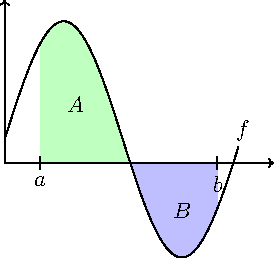
\includegraphics[scale=0.9]{../fig/int6a}\quad
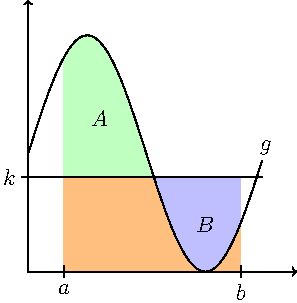
\includegraphics[scale=0.9]{../fig/int6b}
\end{figure}
Forklar ut ifra en arealbetraktning hvorfor\[ \int\limits_a^b f \,dx=\int\limits_a^b g\,dx -(b-a)d  \]
\textbf{b)} Bekreft likheten i oppgave a) ved integrasjon.
\newpage
\op{fogF}
Under vises grafen til $ F(x) $ og $ f(x) $. $ F $ er en antiderivert av $ f $.
\begin{figure}
	\centering
	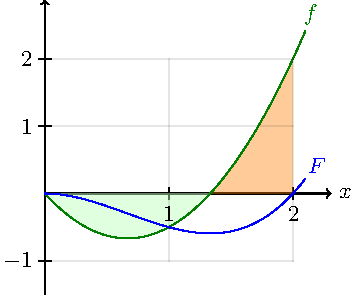
\includegraphics[scale=0.9]{../fig/faropg}\\
	\raggedright
\end{figure}
Forklar hvorfor arealet av det oransje området er like stort som arealet av det grønne området.

\nes
\op{kulevolopg}
La en kule med radius $ r $ være plassert i et koordinatsystem med variabelen $ x $ langs horisontalaksen. Kula er plassert slik at sentrum ligger i origo.\os

\textbf{a)} Lag en tegning og bestem kulas tverrsnitt $ A $ langs horisontalaksen, uttrykt ved $ r $ og $ x $.\os

\textbf{b)} Finn volumet $ V $ av kula.

\op{omdropg} 
Finn volumet av omdreiningslegemene til funksjonene på intervallet $ [0, 1] $:\os

\begin{tabular}{@{}l l l}	
	\textbf{a)} $ f(x)=e^x  $&\quad\textbf{b)} $\displaystyle f(x)= \frac{1}{\sqrt{2}}\sqrt{1-\cos(2 \pi x)}$ &\quad
\end{tabular}
\newpage
\grubop{opgintxkvadmdef}
Bruk definisjonen fra (\ref{bint}) til å vise at
\[ \int\limits_a^b x^2 \,dx = \frac{1}{3}(b^3-a^3) \]
\begin{comment}
\textsl{Hint}: Bruk summen av de naturlige tallene og \eqref{sumkvad} fra s. \pageref{sumkvad}.
\end{comment}

\grubop{opgfunklen}
Gitt en funksjon $ f(x) $ integrerbar på intervallet $ [a, b] $. Vis at \\lengden $ l $ til grafen til $ f $ er
\[ l=\int_{a}^{b} \sqrt{1+g^2}\,dx \]
hvor $ g(x)=f'(x) $.
\fig{opgfunklen}

\begin{comment}
	\subsection*{GeoGebra-oppgaver}
	\op
	Hvis $ |x|\ll 1 $ kan man gjøre følgende tilnærming:
	\[f(x)= \frac{1}{\cos^2 {x}} \approx g(x)=1 + x^2 + \frac{2}{3}x^4 \]
	
	\textbf{a)} Tegn $ f(x) $ og $ g(x) $ inn i et koordinatsystem for $ x\in  [-0.4, 0.4]$
	
	\textbf{b)} Bruk det faktum at $  \int f(x)\, dx = \tan x $ og at $ \int f(x)\, dx \approx \int g(x)\, dx$ for å finne en tilnærming til $ \tan x $
\end{comment}
\end{document}